\lhead{\begin{tikzpicture}[remember picture, overlay]
    \node [anchor=100,inner sep=0] (imagenIZQUIERDA) at (current page header area.north){
\includegraphics[width=18cm]{img/Encabezado.PNG}};
    \end{tikzpicture}}
    \rhead{Flores-Antonio}
    \rfoot{\begin{tikzpicture}[remember picture, overlay]
    \node [anchor=140,inner sep=0] (imagenDERECHA) at (current page footer area.south){
\includegraphics[width=18cm]{img/Foot.PNG}};
    \end{tikzpicture}}
    %----------------------------------------------------------------------------------------
    \lfoot{ \thepage}
    % \renewcommand{\labelenumi}{\alph{enumi}.)} 
    %----------------------------------------------------------------------------------------
    %----------------------------------------------------------------------------------------
    %	TITLE SECTION
    %----------------------------------------------------------------------------------------
    
    \setlength{\droptitle}{-5\baselineskip} % Move the title up
    \title{\textbf{Estudio de tiempos y movimientos en el ensamble de un circuito electrónico utilizando diferentes métodos para su optimización }} % Article title
    
     \author{ 
     \textsc{Apellidos, Nombre/s}\\ 
    %  Afiliación:
     \texttt{ Nombre Instituto } \\ 
     \texttt{Nombre de la Organización } \\ 
     \texttt{Ciudad y País}\\ 
     \texttt{Correo} 
     \and 
     \textsc{Flores Antonio David Ricardo}\\ 
    %  Afiliación:
     \texttt{ Instituto Tecnológico de Querétaro } \\ 
     \texttt{ Tecnológico Nacional de México } \\ 
     \texttt{Querétaro, México}\\ 
     \texttt{daroan13@gmail.com} 
    }
    
    
    %----------------------------------------------------------------------------------------
    
    % \begin{document}
    
    % Print the title
    \maketitle
    \thispagestyle{fancy}
    
    %----------------------------------------------------------------------------------------
    %	ARTICLE CONTENTS
    %----------------------------------------------------------------------------------------
    
    % \section*{Resumen}
    % \textit{Palabras clave:}
    % El resumen (ancho de página) deberá contener entre 100 y 200 palabras tipo Adobe Devangari 11 puntos.
    
    \begin{abstract}
    \noindent 
    El resumen (ancho de página) deberá contener entre 100 y 200 palabras tipo Adobe Devangari 11 puntos.
    
    \end{abstract}
    % 
    % 
    \textbf{\textit{Palabras clave}}: {First keyword should be the corresponding to the research area according with the authors guide. Maximum of 6 keywords.}
    % \keywords{First keyword should be the corresponding to the research area according with the authors guide. Maximum of 6 keywords.}
    
    \section{Introducción}
    
% \begin{itemize}
%     \item Se debe exponer de manera concreta y en lenguaje sencillo : el tema, o lo(s) objeto (s) de estudio. 
%     \item Se deben de mencionar las metodologías más usadas muy brevemente. 
%     \item Se debe de señalar el avance en los últimos años.
%     \item Al final se debe hacer alusión al o lo(s) objetivos del proyecto de investigación.
%     \item Debe de tener Referencias científicas, URL, tesis, etc.
% \end{itemize}
% Define estudio de tiempos y movimientos
El estudio de tiempos y movimientos es una técnica de análisis utilizada en la ingeniería industrial y la gestión de operaciones para mejorar la eficiencia y productividad de los procesos laborales. Este estudio implica dos componentes principales: la medición del tiempo necesario para realizar cada tarea y el análisis de los movimientos realizados durante el trabajo. \cite{Estudiodetiempos}
% define que es ensamble
Un ensamblaje, en el contexto de la producción y la ingeniería, se refiere al proceso de unir o montar varias piezas o componentes individuales para crear un producto final completo. Este término es ampliamente utilizado en diversas industrias, especialmente en la manufactura y la electrónica, donde múltiples partes deben ser ensambladas para formar un dispositivo funcional. \cite{Ensamble}
% define que es un circuito electronico
Un circuito electrónico es una configuración de componentes eléctricos y electrónicos conectados entre sí mediante conductores, que permite el flujo de corriente eléctrica para realizar una función específica. Estos componentes pueden incluir resistencias, condensadores, diodos, transistores, y otros dispositivos que trabajan juntos para procesar señales, realizar cálculos, o controlar otros sistemas. \cite{Circuitoelectrico}
%define optimización
Optimizar hace referencia a la acción y efecto de optimizar. En términos generales, se refiere a la capacidad de hacer o resolver alguna cosa de la manera más eficiente posible y, en el mejor de los casos, utilizando la menor cantidad de recursos. \cite{optimizacion}
% define el metodo de tiempos predeterminados
Para poder realizar el siguiente trabajo utilizaremos el método de tiempos predeterminados, que es una técnica utilizada en el estudio de tiempos y movimientos para establecer estándares de tiempo mediante el uso de datos previamente recopilados y sistematizados sobre los tiempos necesarios para realizar movimientos y tareas básicas. Este método es ampliamente utilizado en la ingeniería industrial para mejorar la eficiencia operativa, planificar la producción y establecer objetivos de rendimiento.
% Al final se debe hacer alusión al o lo(s) objetivos del proyecto de investigación.
El objetivo general de este proyecto de investigación es optimizar el proceso de ensamblaje de circuitos electrónicos mediante el análisis detallado de tiempos y movimientos, con el fin de mejorar la eficiencia, reducir los tiempos de producción, minimizar costos y asegurar una alta calidad en el producto final. Esto incluye varios objetivos específicos, como identificar y eliminar movimientos innecesarios, asegurar que cada paso del proceso se realice de manera eficiente y con alta calidad, y aumentar la productividad implementando métodos más eficientes.
%
%
    \section{Justificación}

% \begin{itemize}
%     \item Se debe de describir lo que se requiere, lo que se necesita o lo que se demanda en la actualidad con un enfoque global pero terminar con menciones a temas locales o nacionales.
%     \item Debe de tener Referencias científicas, URL, tesis, etc.
% \end{itemize}
% 
% Cuantos tipos de manufactura existen?
La manufactura se refiere al proceso de convertir materias primas en productos terminados a través del uso de herramientas, mano de obra, maquinaria y procesos químicos. Existen varios tipos de manufactura, cada uno adecuado para diferentes tipos de productos y necesidades de producción. Cada tipo de manufactura tiene sus propias ventajas y desventajas, y su elección depende de factores como el tipo de producto, la cantidad de producción, los costos, la flexibilidad requerida y la tecnología disponible. \cite{Manufactura}
% Cuantas empresas de manufactura existen en Mundo?
Determinar la cantidad exacta de empresas de manufactura en todo el mundo es un desafío debido a la variedad de definiciones y la constante evolución del sector.
Según un informe de McKinsey, el sector manufacturero representa aproximadamente el 16 del PIB global y el 14 del empleo mundial. En resumen, aunque es difícil proporcionar una cifra exacta, el sector manufacturero es vasto y en expansión, con millones de empresas a nivel mundial contribuyendo significativamente a la economía global. \cite{Empresas}
    % 
    % 
    \section{Descripción del problema}
    % \begin{itemize}
%     \item Se debe describir la desviación o diferencia del ``es'' con respecto al ``debe ser''.
%     \item Se debe hacer alusión a la incógnita científica*.
%     \item Debe de tener Referencias científicas, URL, tesis, etc.
% \end{itemize}
% \textbf{*La incógnita científica es el elemento cuya solución incrementa el conocimiento científico.}
% 
% 
La inversión en educación y tecnología impulsa el progreso nacional, lo que resulta en mejores ingresos para las familias mexicanas y una mayor calidad de vida.
Para competir globalmente, los estudiantes del tecnológico de México deben adquirir competencias en las últimas innovaciones tecnológicas.
El aprendizaje de los alumnos se ve limitado por la falta de tiempo dedicado a las materias y la carencia de habilidades en computación, investigación, trabajo en equipo y trabajo autónomo.
%
%
    \section{Fundamentación teórica}
    
    Es la parte medular y de mayor discusión, deberá ser la fundamentación de la hipótesis, por tanto se deberá señalar claramente la razón de la suposición y fundamentación de la misma. Únicamente referencias científicas.
    \begin{itemize}
        \item Se debe de retomar el tema que se planteo en la introducción, pero ahora profundizando para clarificar la incógnita científica y se pueda plantear la hipótesis.
        \item Se debe de retomar la descripción del problema, pero ahora a profundidad del (los) objeto(s) de estudio. 
        \item Se debe de profundizar en las metodologías que se ha usado para el estudio del tema.
        \item Referencias solo de artículos y libros científicos.
    \end{itemize}
% 
% 
% Cuales son las revoluciones industriales que ha vivido la humanidad?
% A lo largo de la historia del hombre las técnicas manuales para elaborar herramientas y mejorar la caza y la calidad de vida fueron fundamentales para la supervivencia.
% La revolución industrial han cambiado las fuentes de energía básicas y los medios de comunicación para desplazar mercancías, personas e información.
% 
% 
    \section{Hipótesis}
 % Es la suposición con fundamento científico relativa a la solución del problema, necesidad o de cómo se aprovecha la oportunidad con la incógnita científica y se fundamenta con: 1. Una suposición (en afirmativo o negativo) y ésta deberá vincularse con:
% 2. La fundamentación científica que deberá ser precisa 3. Una entidad de comparación para probar la suposición y
% 4. La variable con que se califica o cuantifica la comparación o se prueba la hipótesis.
% 
% 
Desarrollar un proyecto integrador en la materia de estudio del trabajo II implementando todos los temas vistos en la clase incrementara las habilidades del estudiante logrando plantear nuevos proyectos desde cero al determinar el tiempo estándar en el ensamble de un circuito electrónico.
% 
% 
% \begin{itemize}
%     \item Se debe de identificar claramente la suposición científica
%     \item Se debe de identificar claramente el fundamento científico
%     \item Se debe identificar claramente la variable de respuesta
%     \item Se debe identifican claramente las realidades o modelos contrastantes
%     \item Se debe de establecer las variables asociadas, explicativas o que tienen relación funcional con la variable de respuesta
% \end{itemize}
% 
%  
    \section{Objetivo}

% Precisar la acción necesaria para probar la hipótesis. Dicha acción se establece mediante el uso de verbos activos y en infinitivo.
% 
% 
% \begin{itemize}
%     \item Se debe establecer que se pretende probar la hipótesis
% \end{itemize}
% 
%
El objetivo del proyecto es realizar un análisis exhaustivo de los tiempos y movimientos involucrados en el ensamble de circuitos electrónicos, con el fin de identificar áreas de ineficiencia y oportunidades de mejora. A través de este análisis, se buscará implementar métodos y técnicas de optimización que permitan reducir los tiempos de producción, minimizar los movimientos innecesarios de los operarios y mejorar la calidad del producto final.
%
%
    \subsection{Objetivos específicos }

  % \begin{itemize}
%     \item Se debe establecer como un conjunto de acciones comunes para lograr el objetivo general
%     \item Se debe establecer como etapas para lograr el objetivo general
% \end{itemize}

% Son actividades orientadas al cumplimiento del objetivo general. Se establecen con verbos activos en infinitivo. Son parte de la acción encaminada a probar la hipótesis. Éstos deben ser precisos, y en lo posible evitar aspectos metodológicos.
% 
%
\begin{itemize}
        \item Realizar un análisis detallado de los procesos de ensamble de circuitos electrónicos para identificar los pasos críticos y los tiempos asociados a cada actividad.
        \item Evaluar los movimientos realizados por los operarios durante el proceso de ensamble para identificar posibles áreas de mejora en términos de ergonomía y eficiencia.
        \item Investigar y comparar diferentes métodos y técnicas de optimización de tiempos y movimientos utilizados en la industria electrónica.
        \item Seleccionar e implementar las estrategias de optimización más adecuadas para el proceso de ensamble de circuitos electrónicos, considerando factores como la complejidad del proceso y los recursos disponibles.
    \end{itemize} 
    % 
    % 
    \section{Metodología}

El presente trabajo de investigación se llevó a cabo mediante la observación directa y el análisis estadístico de los datos recolectados.
El estudio y la recolección de datos se realizaron en la ciudad de Querétaro, específicamente en las instalaciones del Instituto Tecnológico de Querétaro (ITQ).
La experimentación se desarrolló durante el período comprendido entre febrero y mayo de 2024.
Se eligió el ensamblaje de una tarjeta electrónica como caso de estudio, empleando software de diseño asistido por computadora para definir la estructura en todos sus niveles. Además, se establecieron los límites de potencia y control necesarios para desarrollar la arquitectura adecuada, y se seleccionó la mejor opción para su implementación final. 
En la primera fase de la experimentación, se grabaron dos muestras continuas con una cámara de vídeo de celular, y luego se aplicaron varias metodologías para determinar el tiempo de ciclo y el tiempo estándar.
%
%
\subsection{Desarrollo de la guía de plan de Emergencia}

Un plan de emergencia es un conjunto de procedimientos y acciones predefinidas diseñadas para mitigar, responder y recuperarse de situaciones de emergencia o desastres.\cite{Plan}
\newline
Su objetivo principal es proteger la vida humana, minimizar daños y asegurar una recuperación rápida y efectiva. Un plan de emergencia abarca una variedad de escenarios, incluyendo desastres naturales, incidentes tecnológicos, y emergencias causadas por el hombre.
%
%
\subsection{Análisis de los métodos, materiales, herramientas e instalación utilizada en la ejecución del ensamble de un circuito electrónico}

\subsubsection{Planeación}

Asegúrate de conocer siempre tu objetivo.
Asegúrate de contar con los documentos (formatos, procedimientos, etc).
%
%
\subsubsection{5´s}

Las 5's es una metodología de gestión de calidad originada en Japón que busca mejorar el entorno de trabajo a través de la organización y la estandarización. Su nombre proviene de cinco palabras japonesas que comienzan con la letra "S", y cada una representa un paso fundamental del proceso. La implementación de las 5's puede mejorar la eficiencia, reducir desperdicios, y crear un ambiente de trabajo más seguro y organizado. \cite{5´s}
\newline
Consiste en cinco principios: Seiri (Clasificación), que elimina elementos innecesarios; Seiton (Orden), que organiza los elementos necesarios de manera lógica; Seiso (Limpieza), que mantiene el área de trabajo limpia; Seiketsu (Estandarización), que establece procedimientos para mantener la clasificación, orden y limpieza; y Shitsuke (Disciplina), que fomenta la adherencia continua a estos estándares.
%
%
\subsubsection{Desarrollo del sistema de tiempos predeterminado}
%
%
\subsubsection{Desarrollo del muestreo del trabajo}
%
%
\subsubsection{Corrección por balanceo de procesos}
%
%
\subsubsection{Datos estándar continuos y discretos}
%
%
\begin{figure}[H]
        \centering
        \includegraphics[trim = {40mm 120mm 50mm 100mm},clip,scale=0.2]{10/Img/arduino.pdf}
        \caption{Arduino}
        \label{Arduino}
    \end{figure}

\begin{figure}[H]
        \centering
        \includegraphics[trim = {90mm 45mm 90mm 80mm},clip,scale=0.2]{10/Img/cableUsb.pdf}
        \caption{Cable Usb}
        \label{Cable usbl}
    \end{figure}
    
    \begin{figure}[H]
        \centering
        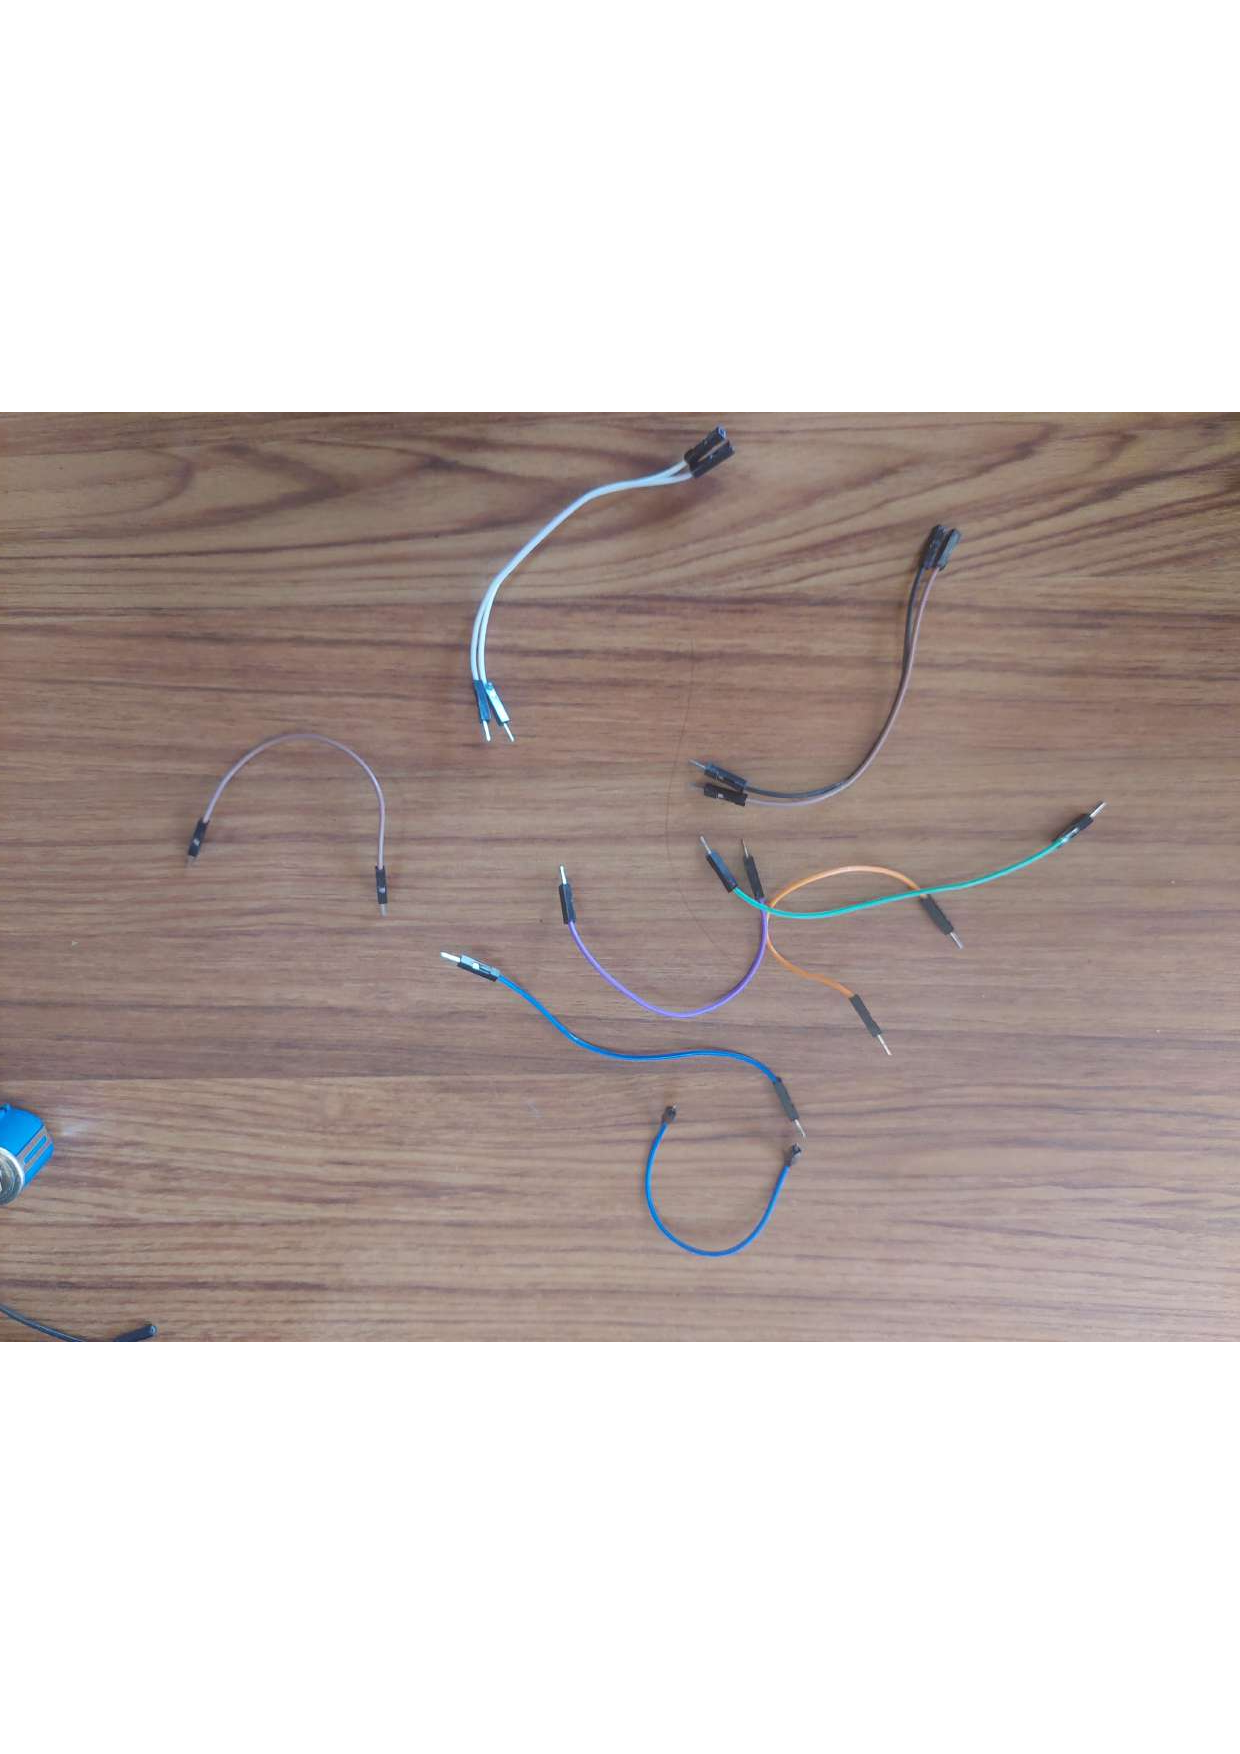
\includegraphics[trim = {30mm 30mm 30mm 30mm},clip,scale=0.2]{10/Img/cablesDupont.pdf}
        \caption{Cables Dupont}
        \label{Cables Dupont}
    \end{figure}
    
    \begin{figure}[H]
        \centering
        \includegraphics[trim = {30mm 30mm 30mm 30mm},clip,scale=0.2]{10/Img/display.pdf}
        \caption{Display}
        \label{Display}
    \end{figure}
    
    \begin{figure}[H]
        \centering
        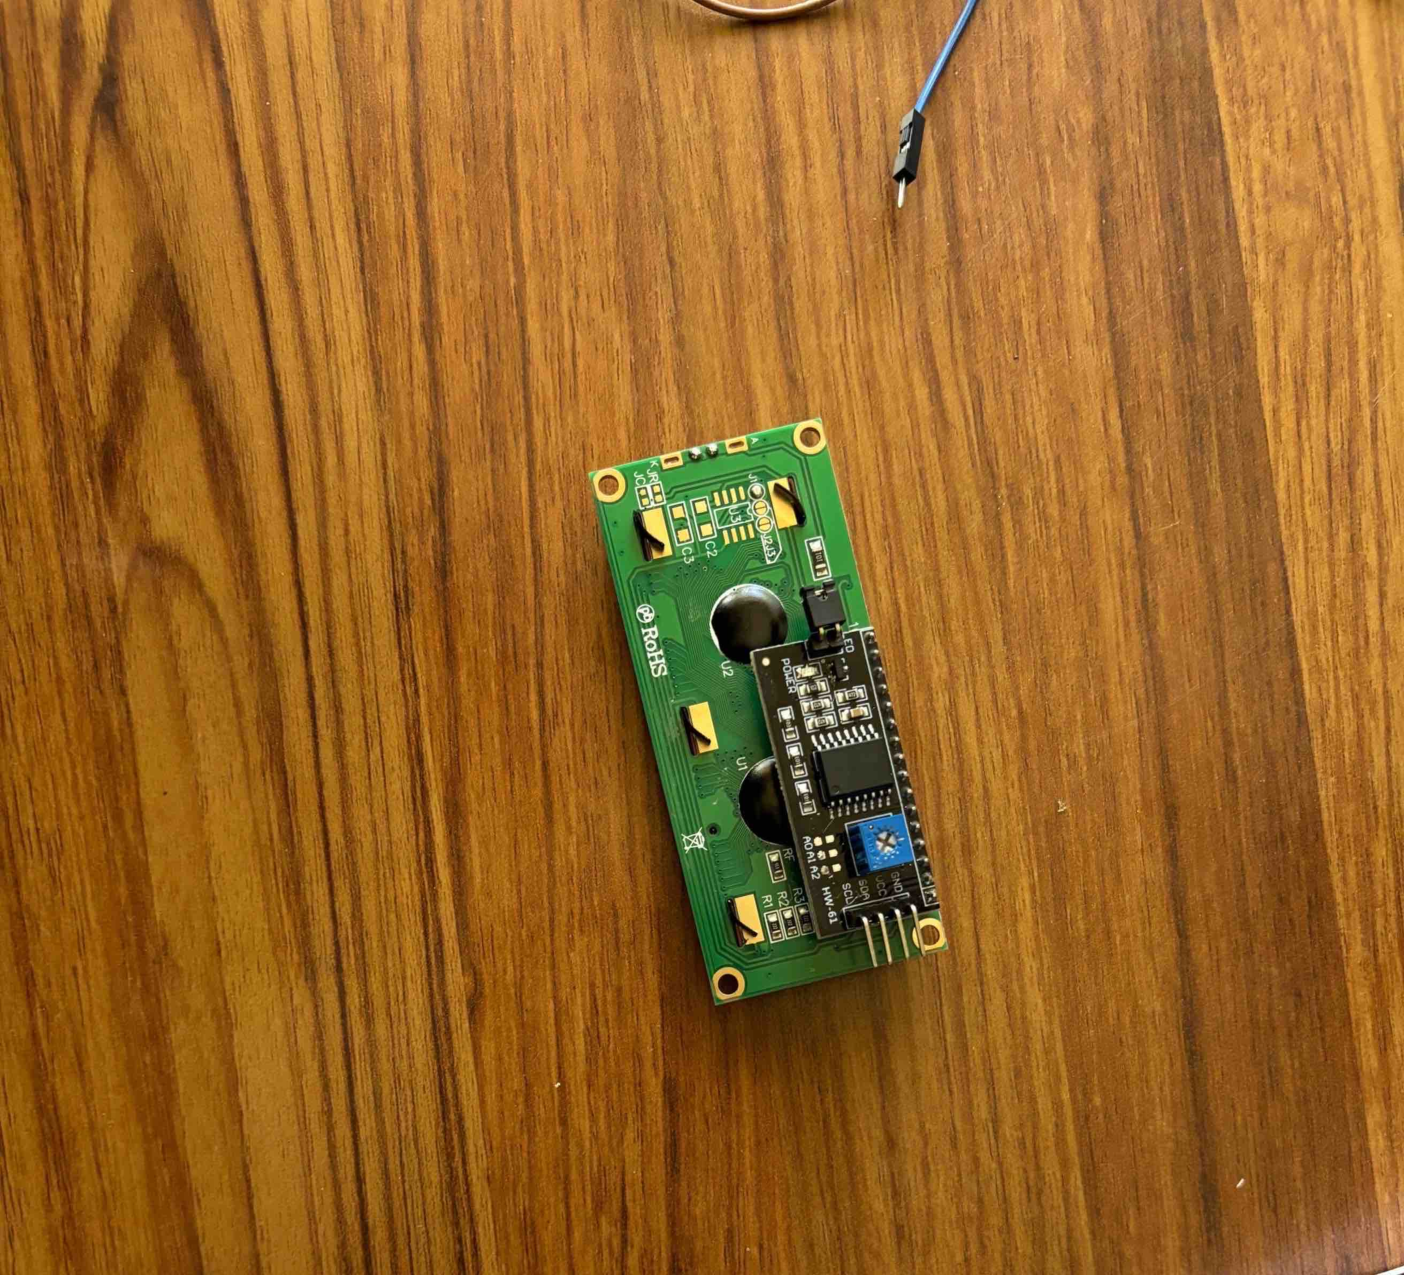
\includegraphics[trim = {30mm 30mm 30mm 30mm},clip,scale=0.2]{10/Img/moduloAdaptador.pdf}
        \caption{Modulo Adaptador}
        \label{Adaptador}
    \end{figure}
    
    \begin{figure}[H]
        \centering
        \includegraphics[trim = {30mm 30mm 30mm 30mm},clip,scale=0.05]{10/Img/multicontacto.pdf}
        \caption{Multicontacto}
        \label{Multicontacto}
    \end{figure}
    
    \begin{figure}[H]
        \centering
        \includegraphics[trim = {30mm 30mm 30mm 30mm},clip,scale=0.2]{10/Img/potenciómetro.pdf}
        \caption{Potenciómetro}
        \label{Potenciómetro}
    \end{figure}
    
    \begin{figure}[H]
        \centering
        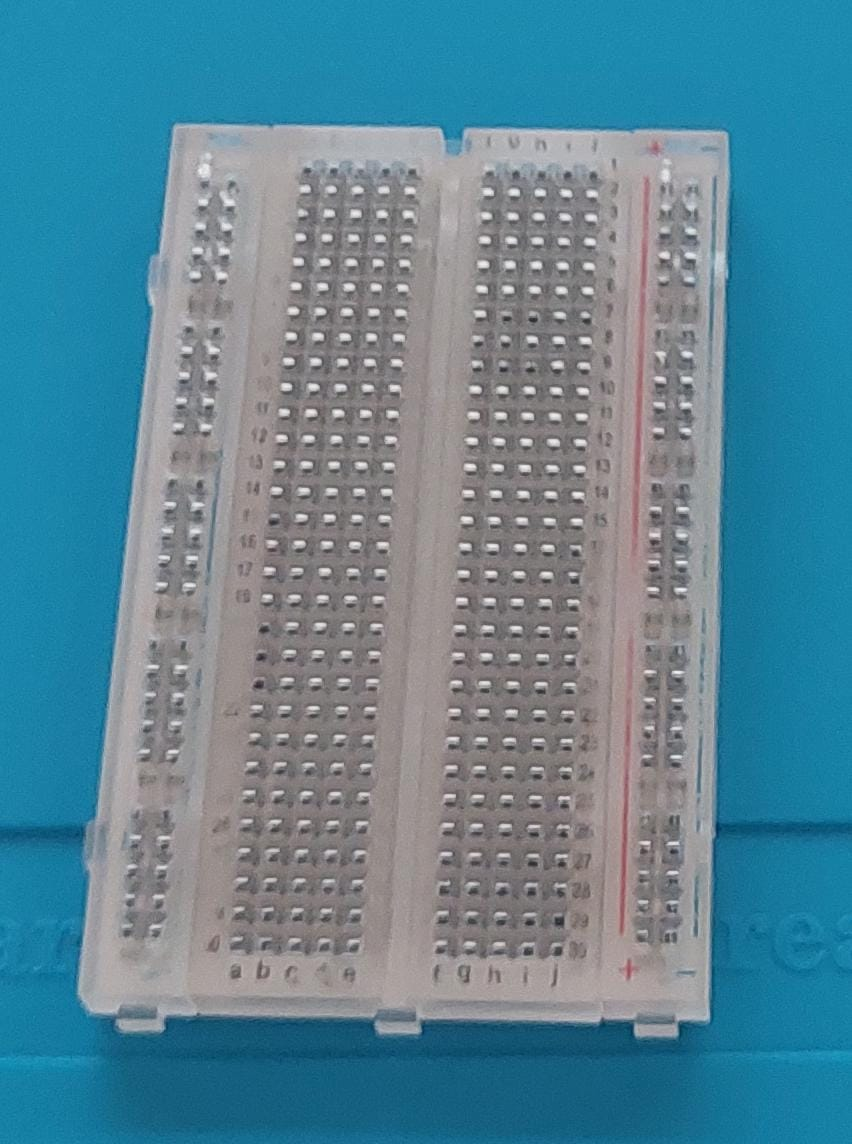
\includegraphics[trim = {10mm 100mm 0mm 0mm},clip,scale=0.2]{10/Img/protoboard.pdf}
        \caption{Protoboard}
        \label{Protoboard}
    \end{figure}
    
    \begin{figure}[H]
        \centering
        \includegraphics[trim = {30mm 30mm 30mm 30mm},clip,scale=0.2]{10/Img/resistencias.pdf}
        \caption{Resistencias}
        \label{Resistencias}
    \end{figure}
%
%

%
%
\subsection{Diseño de la forma más económica de realizar el trabajo}   

%    
%   
\subsection{Normalización de los métodos, materiales, herramientas e instalaciones}    

%
%
\subsection{Determinación del tiempo estándar para que una persona competente realice el trabajo con marcha normal}

%
%
% \subsection{Acrónimos y Abreviaciones}

% Los acrónimos y abreviaciones deberán ser definidos únicamente la primera vez que aparecen en el texto, esto para que el lector entienda lo que significan.

% \subsection{Ecuaciones}

% Las ecuaciones son una excepción a las especificaciones prescritas de esta plantilla. 
% Deberá determinar si su ecuación debe escribirse o no utilizando la fuente Adobe Devangari. 
% Para crear ecuaciones multinivel, puede ser necesario tratar la ecuación como un gráfico e insertarla en el texto después de aplicar el estilo de la platilla.
% Las ecuaciones serán enumeradas de manera consecutiva, y el número de ecuación, entre paréntesis, se colocan al ras de la derecha, utilizando una tabulación derecha.
% 
% \begin{equation}
%     \label{eq1}
%     x + y = z 
% \end{equation}
% 
% Es importante asegurarse de que los símbolos de la ecuación sean definidos antes o inmediatamente después de la ecuación. Utilice “(1)”, en vez de “Eq. 1” al enumerar las ecuaciones, excepto al principio de una oración: “La ecuación (\ref{eq1}) es…”

\section{Resultados y discusión}

\begin{figure}[H]
        \centering
        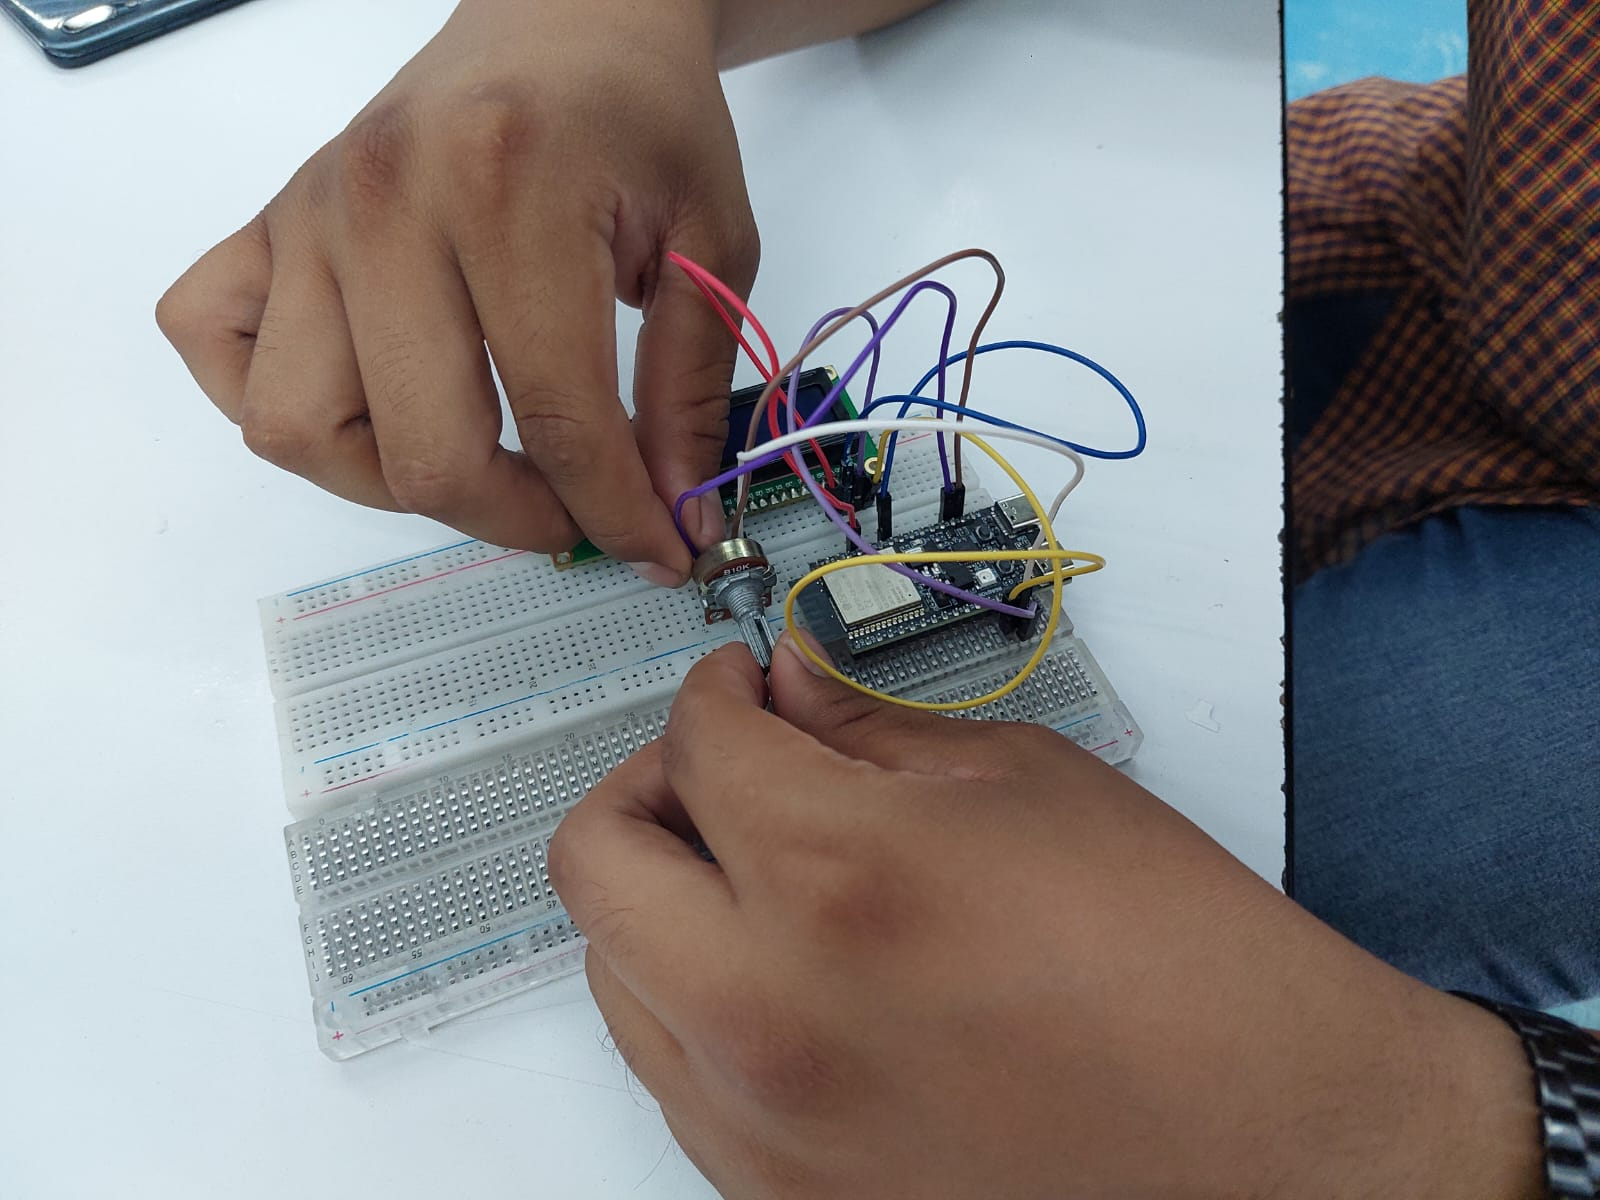
\includegraphics[trim = {30mm 30mm 30mm 30mm},clip,scale=0.2]{10/Img/muestra1Prueba1.jpg}
        \caption{Primera muestra. Prueba 1}
        \label{Prueba 1}
    \end{figure}

\begin{figure}[H]
        \centering
        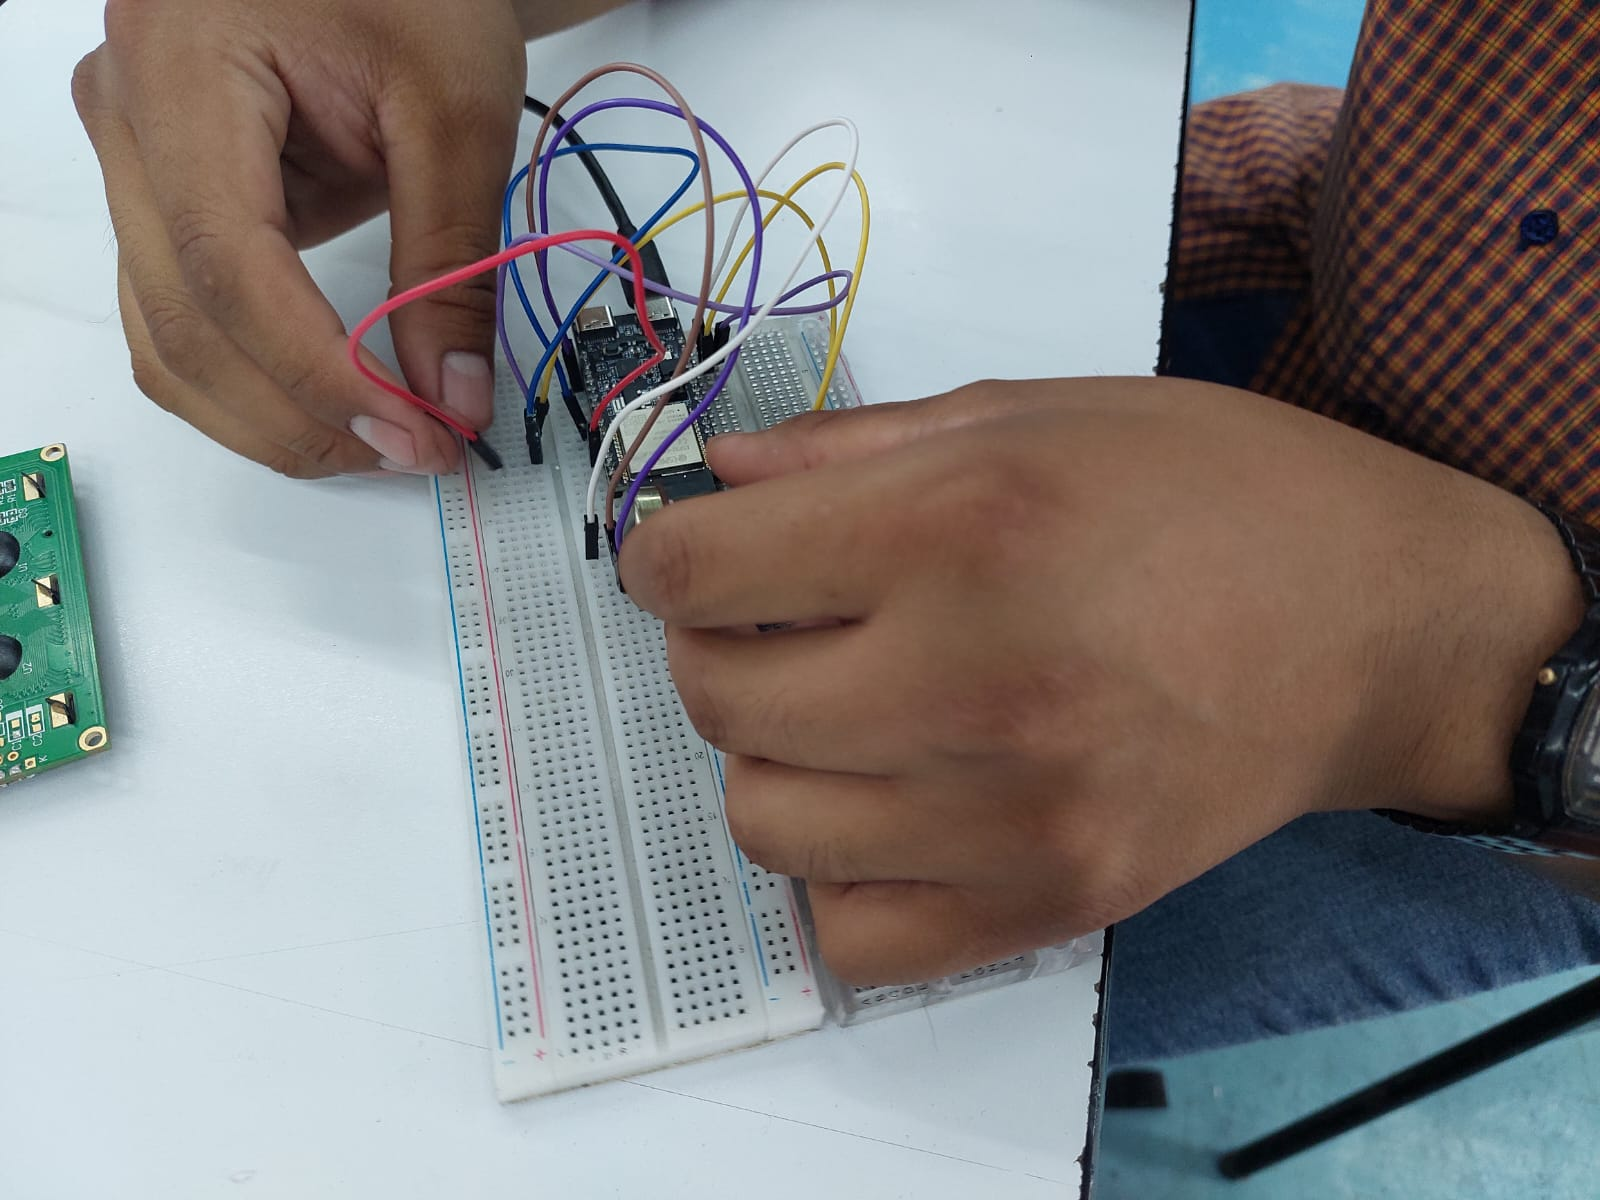
\includegraphics[trim = {30mm 30mm 30mm 30mm},clip,scale=0.2]{10/Img/muestra1Prueba2.jpg}
        \caption{Primera muestra. Prueba 2}
        \label{Prueba 2}
    \end{figure}

\begin{figure}[H]
        \centering
        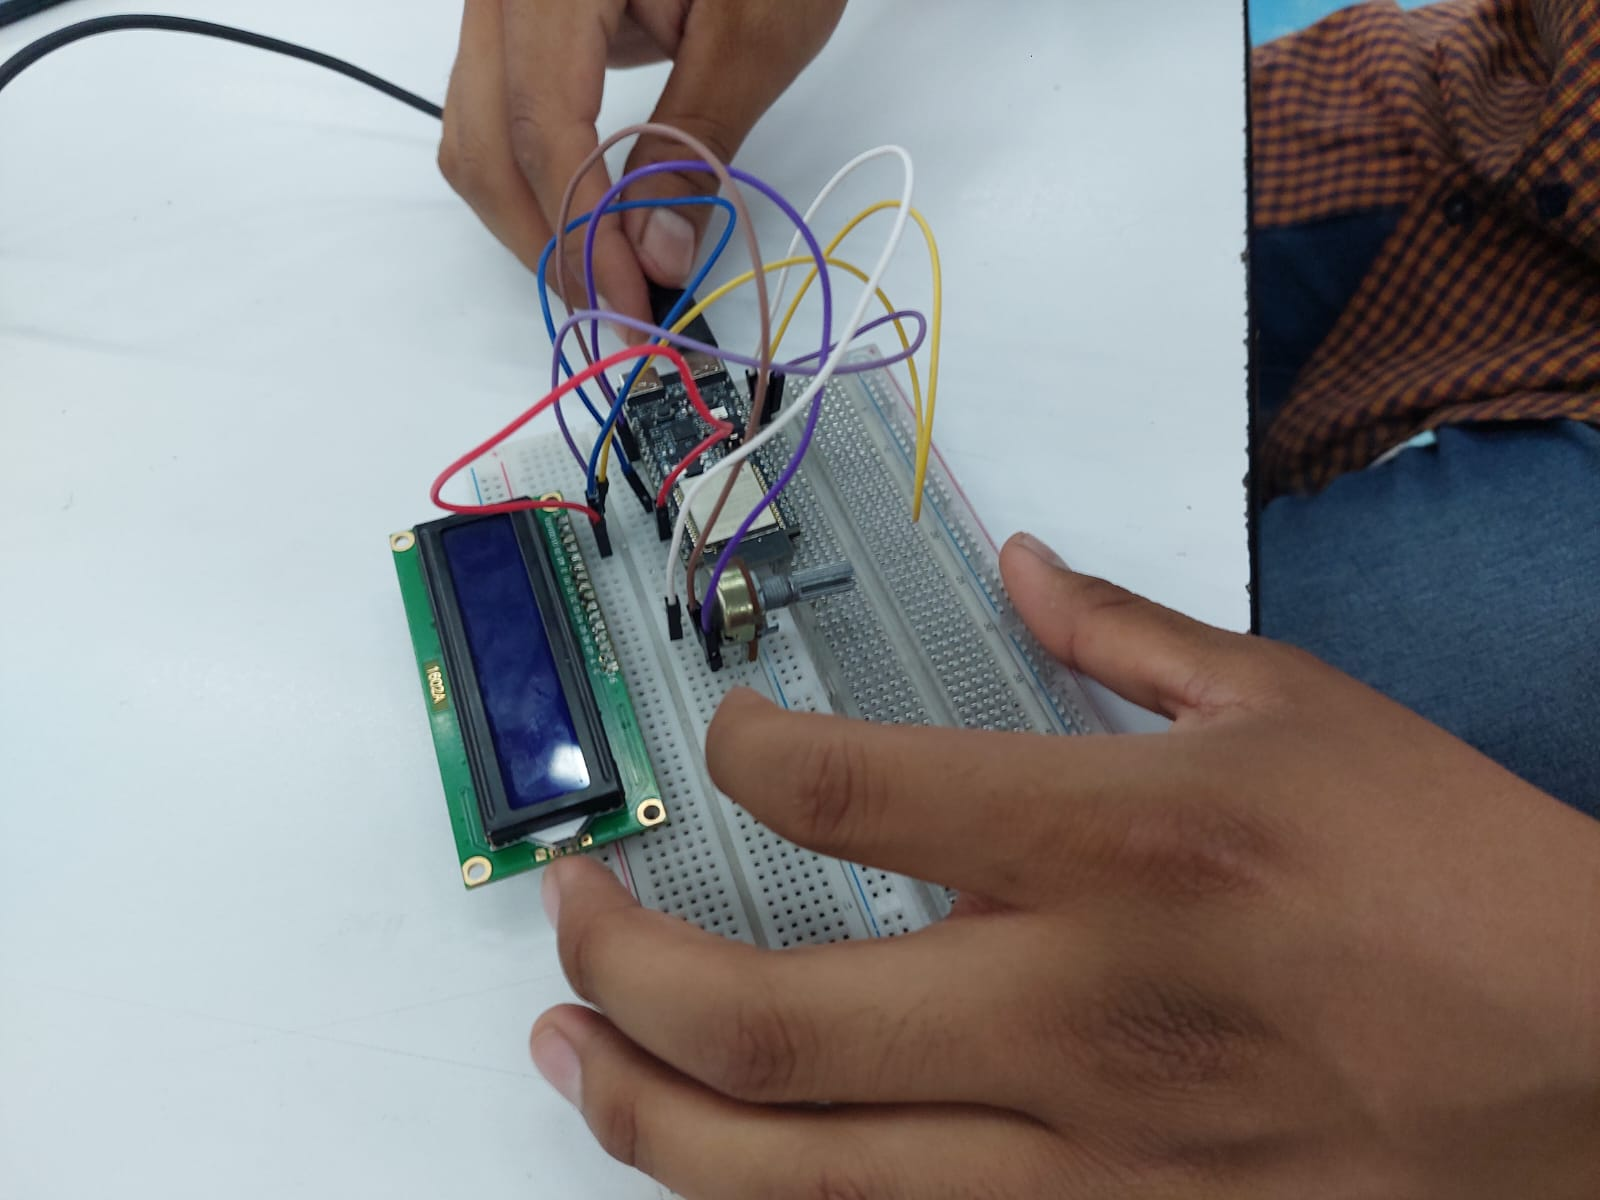
\includegraphics[trim = {30mm 30mm 30mm 30mm},clip,scale=0.2]{10/Img/muestra1Prueba3.jpg}
        \caption{Primera muestra. Prueba 3}
        \label{Prueba 3}
    \end{figure}

\begin{figure}[H]
        \centering
        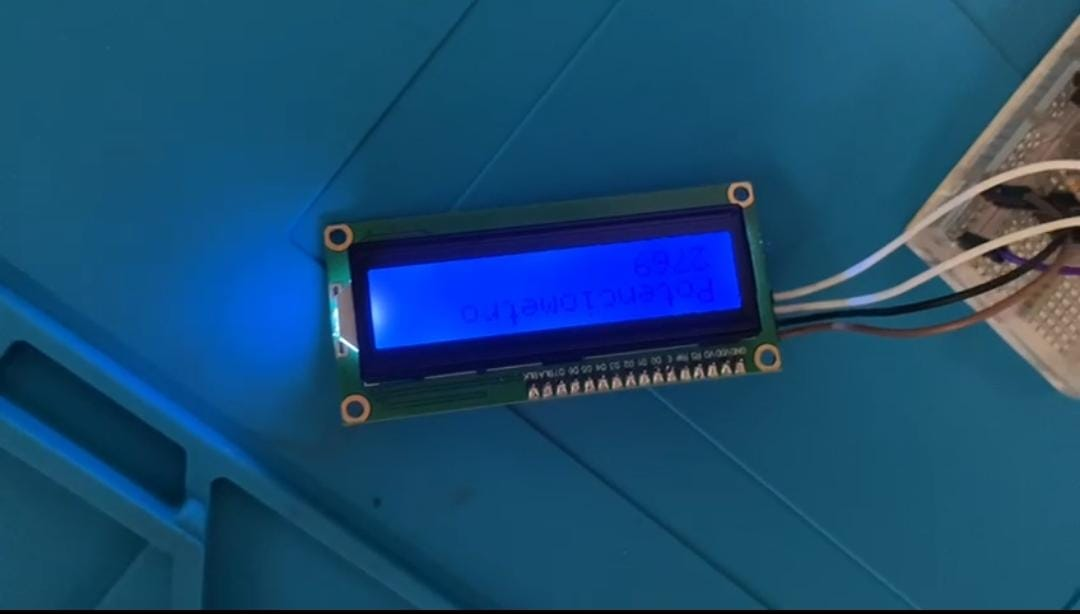
\includegraphics[trim = {30mm 30mm 80mm 30mm},clip,scale=0.2]{10/Img/muestra1Prueba4.jpg}
        \caption{Primera muestra. Prueba 4}
        \label{Prueba 4}
    \end{figure}

\begin{figure}[H]
        \centering
        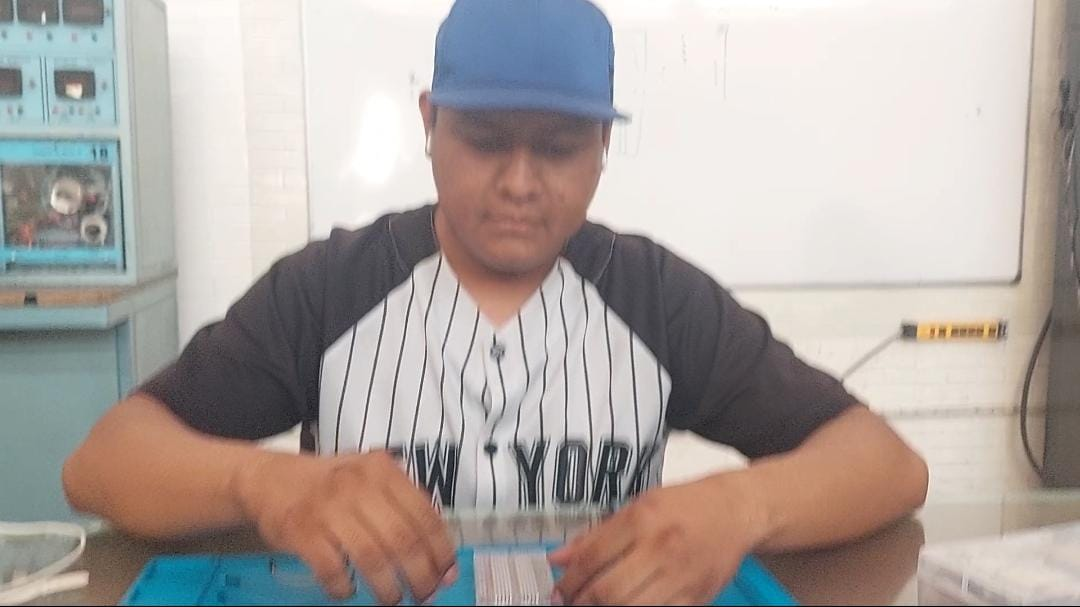
\includegraphics[trim = {30mm 30mm 30mm 30mm},clip,scale=0.2]{10/Img/muestra2Prueba1.jpg}
        \caption{Segunda muestra. Prueba 1}
        \label{Prueba 2.1}
    \end{figure}

\begin{figure}[H]
        \centering
        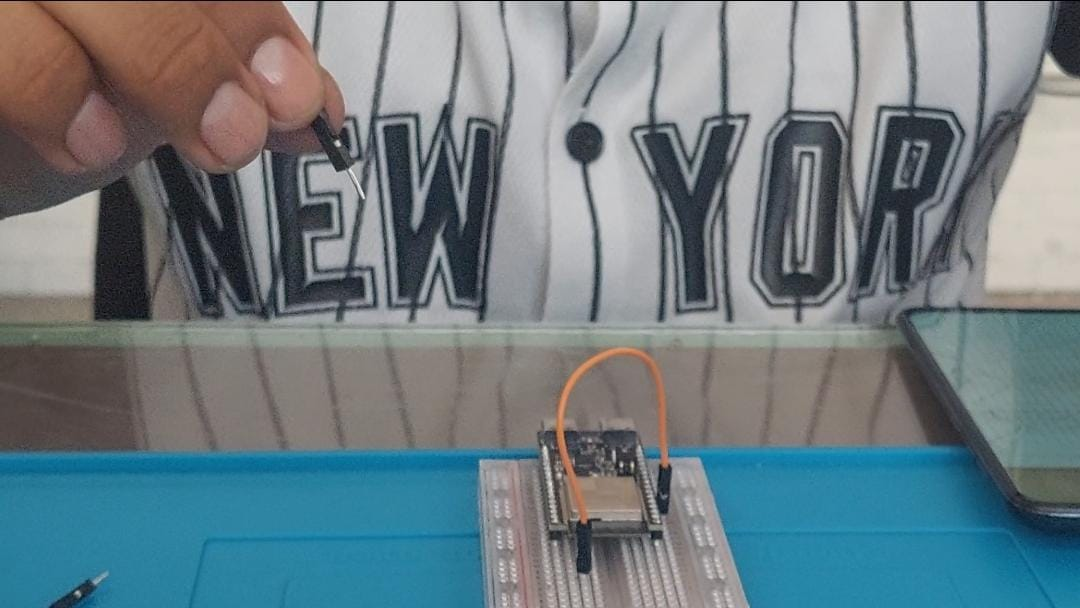
\includegraphics[trim = {30mm 30mm 30mm 30mm},clip,scale=0.2]{10/Img/muestra2Prueba2.jpg}
        \caption{Segunda muestra. Prueba 2}
        \label{Prueba 2.2}
    \end{figure}

\begin{figure}[H]
        \centering
        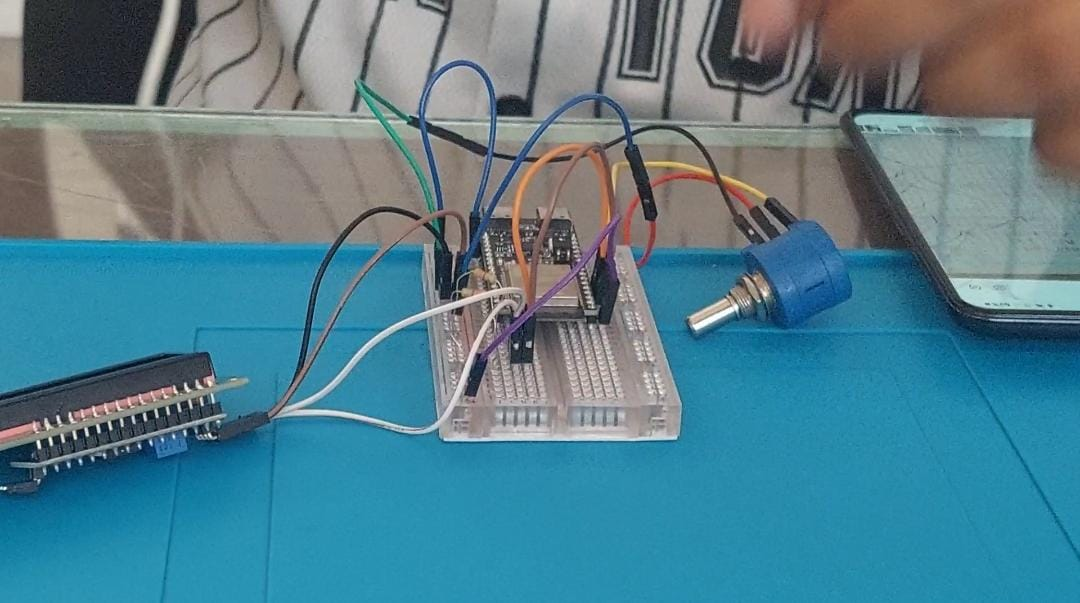
\includegraphics[trim = {30mm 30mm 30mm 30mm},clip,scale=0.2]{10/Img/muestra2Prueba3.jpg}
        \caption{Segunda muestra. Prueba 3}
        \label{Prueba 2.3}
    \end{figure}

\begin{figure}[H]
        \centering
        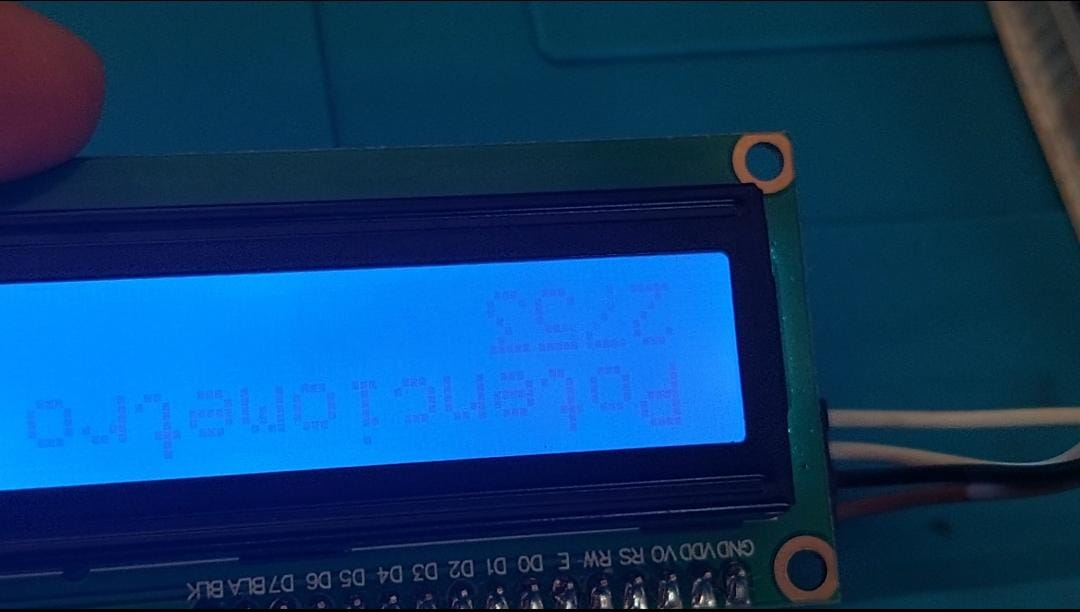
\includegraphics[trim = {30mm 30mm 30mm 30mm},clip,scale=0.2]{10/Img/muestra2Prueba4.jpg}
        \caption{Segunda muestra. Prueba 4}
        \label{Prueba 2.4}
    \end{figure}

\subsection{Desarrollo de la guía de plan de Emergencia}

Esta guía tiene como objetivo eliminar completamente las emergencias relacionadas con incendios y reducir el riesgo de accidentes en el Instituto Tecnológico de Querétaro. Para lograrlo, se identificará al personal que ha recibido capacitación al menos una vez al año, asegurando que, en caso de emergencia, puedan tomar las mejores decisiones para proteger la integridad física de todos, tanto dentro como fuera de la institución, y salvaguardar las instalaciones.
%
%
\subsubsection{Objetivo}

El objetivo del proyecto es realizar un análisis exhaustivo de los tiempos y movimientos involucrados en el ensamble de circuitos electrónicos, con el fin de identificar áreas de ineficiencia y oportunidades de mejora. A través de este análisis, se buscará implementar métodos y técnicas de optimización que permitan reducir los tiempos de producción, minimizar los movimientos innecesarios de los operarios y mejorar la calidad del producto final.
%
%
\subsubsection{Datos Generales del Establecimiento}

\begin{itemize}
    \item\textbf{Nombre comercial:} Instituto Tecnológico de Querétaro (ITQ)
    \item\textbf{Domicilio:} Av. Tecnológico s/n esq. Gral. Mariano Escobedo. Colonia Centro Histórico C.P. 76000, Querétaro, Qro. Figura \ref{fig:plano.png}
    \item\textbf{Teléfonos:} (442) 227 44 00 Ext. 4423
    \item\textbf{Horario de servicio:}
    \item\textbf{Actividad principal:} Su actividad principal es ofrecer programas académicos de nivel superior, incluyendo licenciaturas, ingenierías, maestrías y doctorados, orientados a la preparación de recursos humanos altamente calificados para satisfacer las necesidades del sector industrial y tecnológico.
    \item\textbf{Representante legal:} 
    \item\textbf{Cantidad de trabajadores:} 
    \item\textbf{Superficie del establecimiento:} 78,575 m2
\end{itemize}
%
%
\subsubsection{Plano de localización}
%
%
\begin{figure}[H]
    \centering
    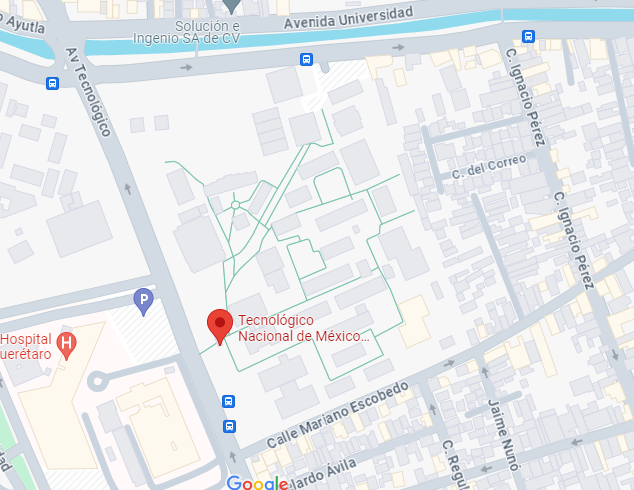
\includegraphics[scale=0.4]{10/Img/plano.png}
    \caption{Instituto Tecnológico de Querétaro}
    \label{fig:plano.png}
\end{figure}
%
%
\subsubsection{Análisis de riesgos}

El riesgo se define como la combinación de la probabilidad de que se produzca un evento y sus consecuencias negativas. Los factores que lo componen son la amenaza y la vulnerabilidad.\cite{Riesgo}
\newline
El análisis de riesgos es un proceso fundamental para identificar, evaluar y priorizar los riesgos que pueden afectar a una organización, proyecto o cualquier otro ámbito en el que se desarrolle una actividad. Este proceso ayuda a tomar decisiones informadas para mitigar, transferir, aceptar o evitar dichos riesgos. 
\begin{table}[h]
        \centering
        \caption{Riesgos con diferentes niveles y colores para distinguir la gravedad y acciones}
        \begin{tabular}{c c c}
        \hline
        \multicolumn{3}{c}{\textbf{Riesgos}}\\
        \hline
             Alto& 0.99 - 0.18 & Rojo  \\
        \hline
             Medio& 0.17 - 0.05 & Amarillo  \\
        \hline
             Bajo& 0.04 - 0.01 & Verde \\
        \hline     
        \end{tabular}
        \label{tab:riego}
    \end{table}
%
%
\subsubsection{Identificación de riesgos internos}

Los riesgos internos de una empresa son todos aquellos que dependen de nuestra gestión dentro de la Empresa y de los distintos departamentos que la componen. \cite{Riesgos}
%
%
\begin{figure}[H]
    \centering
    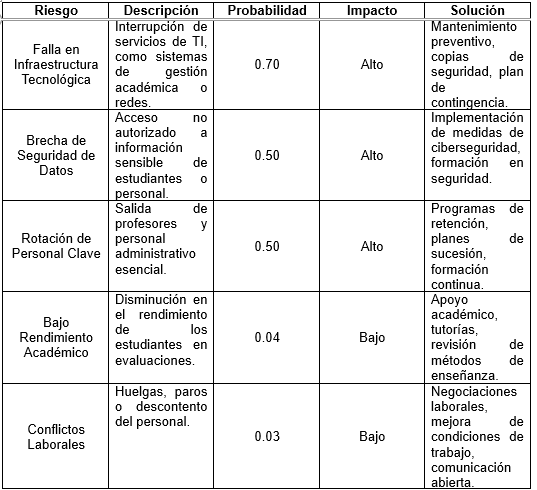
\includegraphics[scale=0.4]{10/Img/riesgosInternos.png}
    \caption{Riesgos Internos en una universidad}
    \label{fig:riesgosInternos.png}
\end{figure}
%
%
\subsubsection{Identificación de riesgos externos}

Los riesgos externos de una empresa son todos aquellos que provienen del entorno de la Empresa y que influyen o condicionan su operativa pudiendo convertirse en amenazas para su desarrollo. \cite{Riesgos}
%
%
\begin{figure}[H]
    \centering
    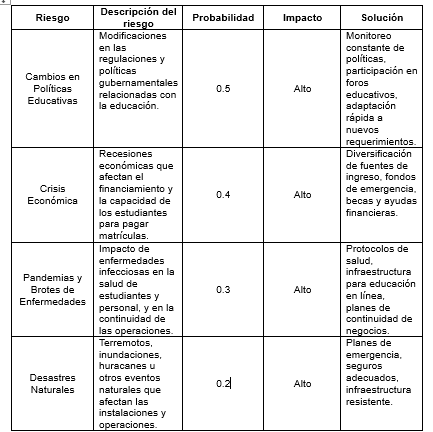
\includegraphics[scale=0.4]{10/Img/riesgosExternos.png}
    \caption{Riesgos Externos en una universidad}
    \label{fig:riesgosExternos.png}
\end{figure}
%
%
\subsubsection{Programa de actividades de prevención y auxilio}

Declaramos las diferentes acciones de lo que se piensa hacer cuando ocurra un riesgo interno u externo. 
Las actividades de preparación y disposición que se hace anticipadamente en el ITP para evitar riesgos.
% 
% 
\subsubsection{Plan de acción}

Es el conjunto unitario de instrucciones que permite al ITQ realizar funciones diversas, como la resolución de problemas referentes a el manejo de riesgos internos y externos.
%
%
\subsubsection{Identificación de capacidades}

\begin{table}[H]
    \centering
    \caption{Recursos en materia de seguridad}
    \begin{tabular}{c c c}
    \hline
    \multicolumn{3}{c}{Inventario de recursos en materia de seguridad}\\
    \hline
         No.& Recurso & Cantidad  \\
    \hline
         1& Extintor & 39  \\
    \hline
         2& Botiquín & 0  \\
    \hline
         3& Detector de humo & 0 \\
    \hline
         4& Lampara de emergencia & 0 \\
    \hline     
    \end{tabular}
    \label{tab:inventario}
\end{table}
%
%
\subsubsection{Plano de localización de recursos}
%
%
\begin{figure}[H]
        \centering
        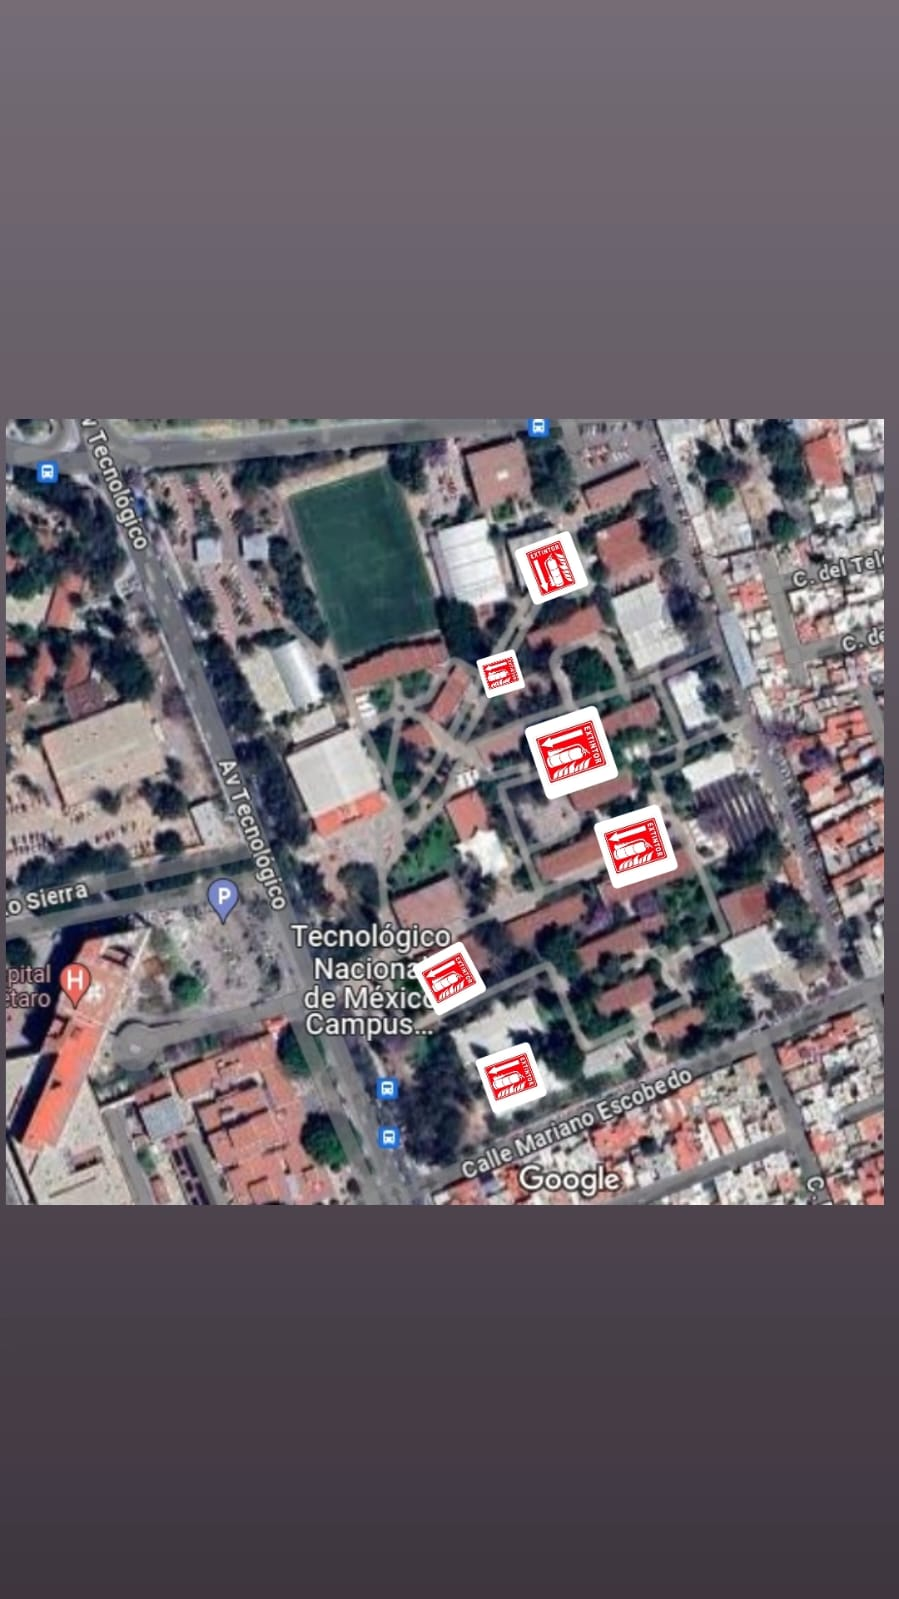
\includegraphics[trim = {30mm 120mm 30mm 120mm},clip,scale=0.2]{10/Img/recursos.jpg}
        \caption{Identificación de extintores}
        \label{Recursos}
    \end{figure}
%
%
\subsubsection{ Identificación de apoyos externos}

    \begin{itemize}
        \item Se debe establecer que se habrá de hacer, como, conque, y donde para obtener la información que permita probar la hipótesis.  
        \item Se debe desglosar de acuerdo a los objetivos específicos. 
        \item Se debe establecer una estrategia metodológica por cada objetivo específico. De manera simplista se podría decir que se cambia el verbo en infinitivo por su respectivo adverbio.
        \item En cada objetivo se debe describir que método, que materiales y que equipo se usará para conseguirlo.
        \item Se deben tener referencias Figura 
    \end{itemize}
    % 
    % 
    % \begin{figure}[H]
        % \centering
    
    % 
    % 
    \subsection{Prepara tu documento}
    
    Antes de que comiences a utilizar esta plantilla, es recomendable que prepare la información que contendrá en un archivo aparte. 
    Ten preparadas tus gráficas, así como también las tablas aparte, para que sea más fácil integrarlo. 
    Se recomienda fuertemente el uso de \textbf{formato Enhanced Metafile (.emf) para imágenes y gráficas} de resolución óptima. 
    Finalmente, completa y organiza el contenido antes de darle el formato de esta plantilla. 
    
    \subsection{Acrónimos y Abreviaciones}
    
    Los acrónimos y abreviaciones deberán ser definidos únicamente la primera vez que aparecen en el texto, esto para que el lector entienda lo que significan.
    
    \subsection{Ecuaciones}
    
    Las ecuaciones son una excepción a las especificaciones prescritas de esta plantilla. 
    Deberá determinar si su ecuación debe escribirse o no utilizando la fuente Adobe Devangari. 
    Para crear ecuaciones multinivel, puede ser necesario tratar la ecuación como un gráfico e insertarla en el texto después de aplicar el estilo de la platilla.
    Las ecuaciones serán enumeradas de manera consecutiva, y el número de ecuación, entre paréntesis, se colocan al ras de la derecha, utilizando una tabulación derecha. 
    
    \begin{equation}
        \label{eq1}
        x + y = z 
    \end{equation}
    
    Es importante asegurarse de que los símbolos de la ecuación sean definidos antes o inmediatamente después de la ecuación. Utilice “(1)”, en vez de “Eq. 1” al enumerar las ecuaciones, excepto al principio de una oración: “La ecuación (\ref{eq1}) es…”
    
    \section{Resultados y discusión}
    
    Antes de comenzar a preparar tu artículo, es importante que lea primero la guía del autor, la cual incluye los temas o apartados que son necesarios para tener tu trabajo completo.
    Una vez completada la edición del texto, el documento está listo para el uso de esta plantilla. En este archivo recién creado, resalte todo el contenido e importe el archivo de texto preparado. Ahora esta listo para estilizar su documento.
    En esta sección se deben presentar todo lo obtenido de la sección 2, incluidas deducciones o efectos del desarrollo. También se podrán incluir subsecciones numeradas de la siguiente forma:
    
    \subsection{Autores y Afiliaciones}
    
    Para distinguir las afiliaciones de los autores, utilice superíndices iniciando con el número 1, 2, etc., sucesivamente, esto dependerá de la cantidad de los departamentos a los que estén afiliados los autores. En caso de que todos los autores pertenezcan a una mismo departamento e institución, utilizar sólo el superíndice 1. 
    
    \subsection{Identificar los encabezados}
    
    Se les recuerda a los autores que los encabezados deben de estar conforme los solicita la guía del autor. De ahí se puede adaptar el trabajo para que sea más fácil de entender para el lector.
    Los encabezados organizan los temas sobre una base relacional y jerárquica. Por ejemplo, el título del documento es encabezado del texto principal porque todo el material posterior se relaciona y elabora sobre este tema. 
    
    \subsection{Tablas y Figuras}
  
    
    \begin{enumerate}
        \item Posición de las tablas y figuras: Coloque las figuras y las tablas en la parte superior e inferior de las columnas. Evite colocarlos en medio. Las figuras y las tablas grandes pueden abarcar ambas columnas. Los títulos de las figuras deben de estar debajo de las mismas; los títulos de las tablas deben aparecer encima de ellas. Insértese las figuras y los cuadros después de citarse en el texto. Utilice la abreviatura “Fig. 1”, incluso al principio de una oración. 
    \end{enumerate}
    
    \section{Conclusiones}
    
    Se describe aquí el alcance del trabajo, logros obtenidos y perspectivas para el futuro de este. Se sugiere colocar información cuantitativa obtenida.
    
    \section{Agradecimientos}
    
    Es importante darles su debido reconocimiento a los laboratorios, instituciones, organizaciones, entre otros que han sido participes para la culminación de este trabajo. También es importante mencionar, fondos, proyectos, becas, entre otros que se le han otorgado al o los autores para realizar el trabajo de investigación. Ejemplo: “Los autores agradecen al Concejo Nacional de Ciencia y Tecnología por los recursos otorgados…”
    
    \section*{Referencias}
    
    Para esta platilla, se solicita al autor enumerar las citas de manera consecutiva entre corchetes 
    La puntuación de la oración que sigues sería  
    Refiérase simplemente al número de referencia, como en , no utilice “Ref. [3]” o “referencia [3]” excepto al principio de una oración: “La referencia [3] fue la primera…”
    Enumere las notas al pie por separado en superíndices. Coloque la nota de pie de en la parte inferior de la columna en la que se citó. No coloque notas al pie en la lista de referencias. Utilice letras para las notas al pie de la tabla.
    A menos de que haya tres autores o más; no utilice “et al.”. Los trabajos que no hayan sido publicados, incluso si han sido presentados para su publicación, deben ser citados como “inéditos”. Los trabajos que han sido aceptados para su publicación deben de citarse como “en prensa”. Poner en mayúscula sólo la primera palabra de un título, excepto los nombres propios y los símbolos de elemento. 
    Otros ejemplos 
    Véase el link  Véase el Apéndice 
    
    % Ejemplo
    %  @Article{article,
    % 	author = "Author1 LastName1 and Author2 LastName2 and Author3 LastName3",
    % 	title = "Article Title",
    % 	volume = "30",
    % 	number = "30",
    % 	pages = "10127-10134",
    % 	year = "2013",
    % 	doi = "10.3389/fnins.2013.12345",
    % 	URL = "http://www.frontiersin.org/Journal/10.3389/fnins.2013.12345/abstract",
    % 	journal = "Frontiers in Neuroscience"
    % }
    
    % @book{book,
    %   author    = {Author Name}, 
    %   title     = {The title of the work},
    %   publisher = {The name of the publisher},
    %   address   = {The city},
    %   year      = 1993,
    % }
    
    % @incollection{chapter,
    %   author       = {Bauthor Surname}, 
    %   title        = {The title of the work},
    %   editor       = {Editor Name},
    %   booktitle    = {The title of the book},
    %   publisher    = {The name of the publisher},
    %   address      = {The city},
    %   year         = 2002,
    %   pages        = {201-213},
    % }
    
    % @InProceedings{conference,
    %   author = {Cauthor Name and Dauthor Surname and Fauthor LastName},
    %   title = {The title of the work},
    %   booktitle = {The title of the conference proceedings},
    %   year = 1996,
    %   publisher = {The name of the publisher},
    %   editor = {Editor Name1 and Editor Name2},
    %   pages = {41-50},
    % }
    
    % @book{cho,
    %   author       = {Gauthor Name1}, 
    %   title        = {The title of the work},
    %   publisher = {Country code and patent number},
    %   address      = {Patent Country},
    %   year = 2013
    % }
    
    % @book{patent,
    %   author    = {Hauthor Surname1}, 
    %   title     = {The title of the work},
    %   publisher = {Patent number},
    %   address   = {Patent country},
    %   year      = 2010,
    % }
    
    % % please use misc for datasets
    % @misc{dataset, 
    % 	author = "Author1 LastName1 and Author2 LastName2 and Author3 LastName3",
    % 	title = "Data Title",
    % 	year = "2011",
    % 	doi = "10.000/55555",
    % 	URL = "http://www.frontiersin.org/",
    % }

    \newpage
    \bibliographystyle{ieeetr}
    \bibliography{10/referencias}
    % 
    % 
    % 
    %%%%%%%%%%%%%%%%%%%%%%%%%%%%%%%%%%
    %\appendix
    %%%%%%%%%%%%%%%%%%%%%%%%%%%%%%%%%%
    % 
    % 
    \centering{\section[\appendixautorefname{}]{Apéndice}}\label{material}
    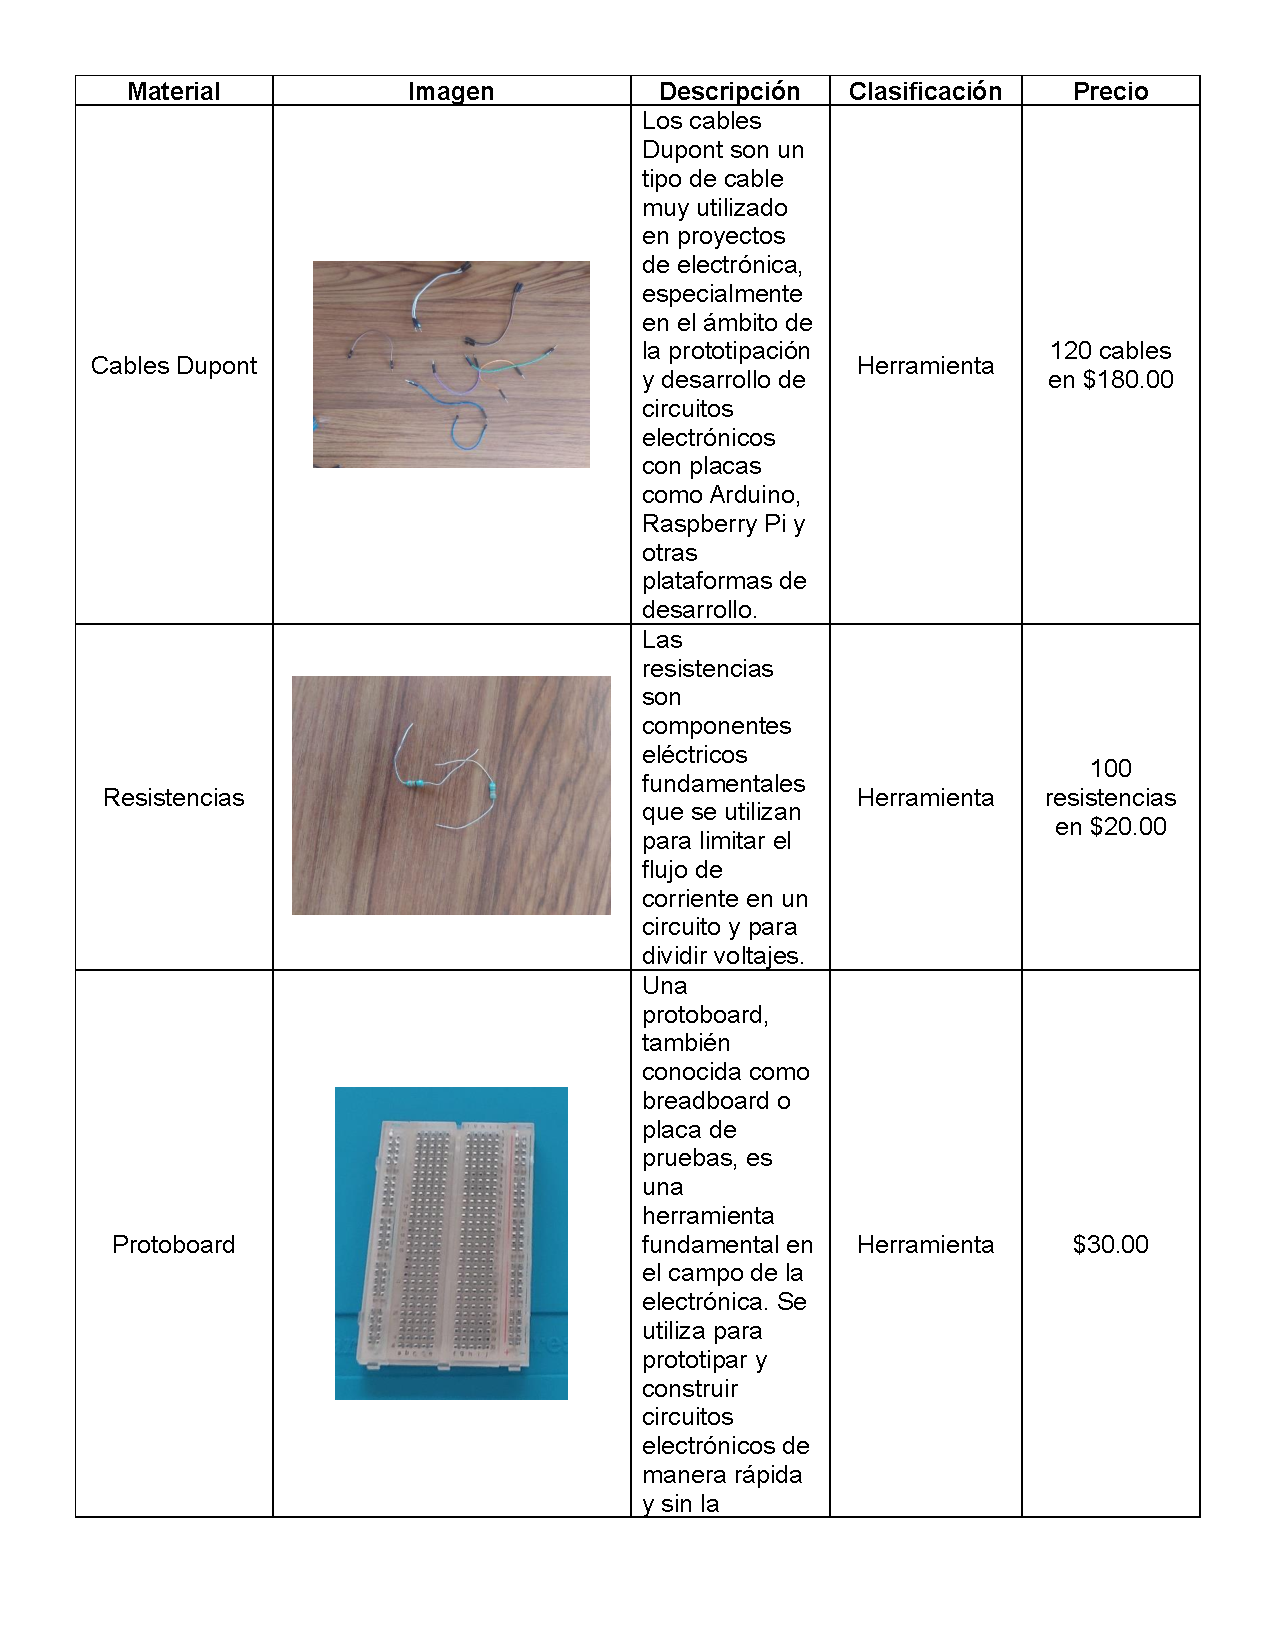
\includepdf[pages=-]{10/Img/material.pdf}
    %%%%%%%%%%%%%%%%%%%%%%%%%%%%%%%%%%%%%%%%
    %%%%%%%%%%%%%%%%%%%%%%%%%%%%%%%%%%
    %\appendix
    %%%%%%%%%%%%%%%%%%%%%%%%%%%%%%%%%%
    % 
    % 
    \centering{\section[\appendixautorefname{}]{Apéndice}}\label{mensamblel}
    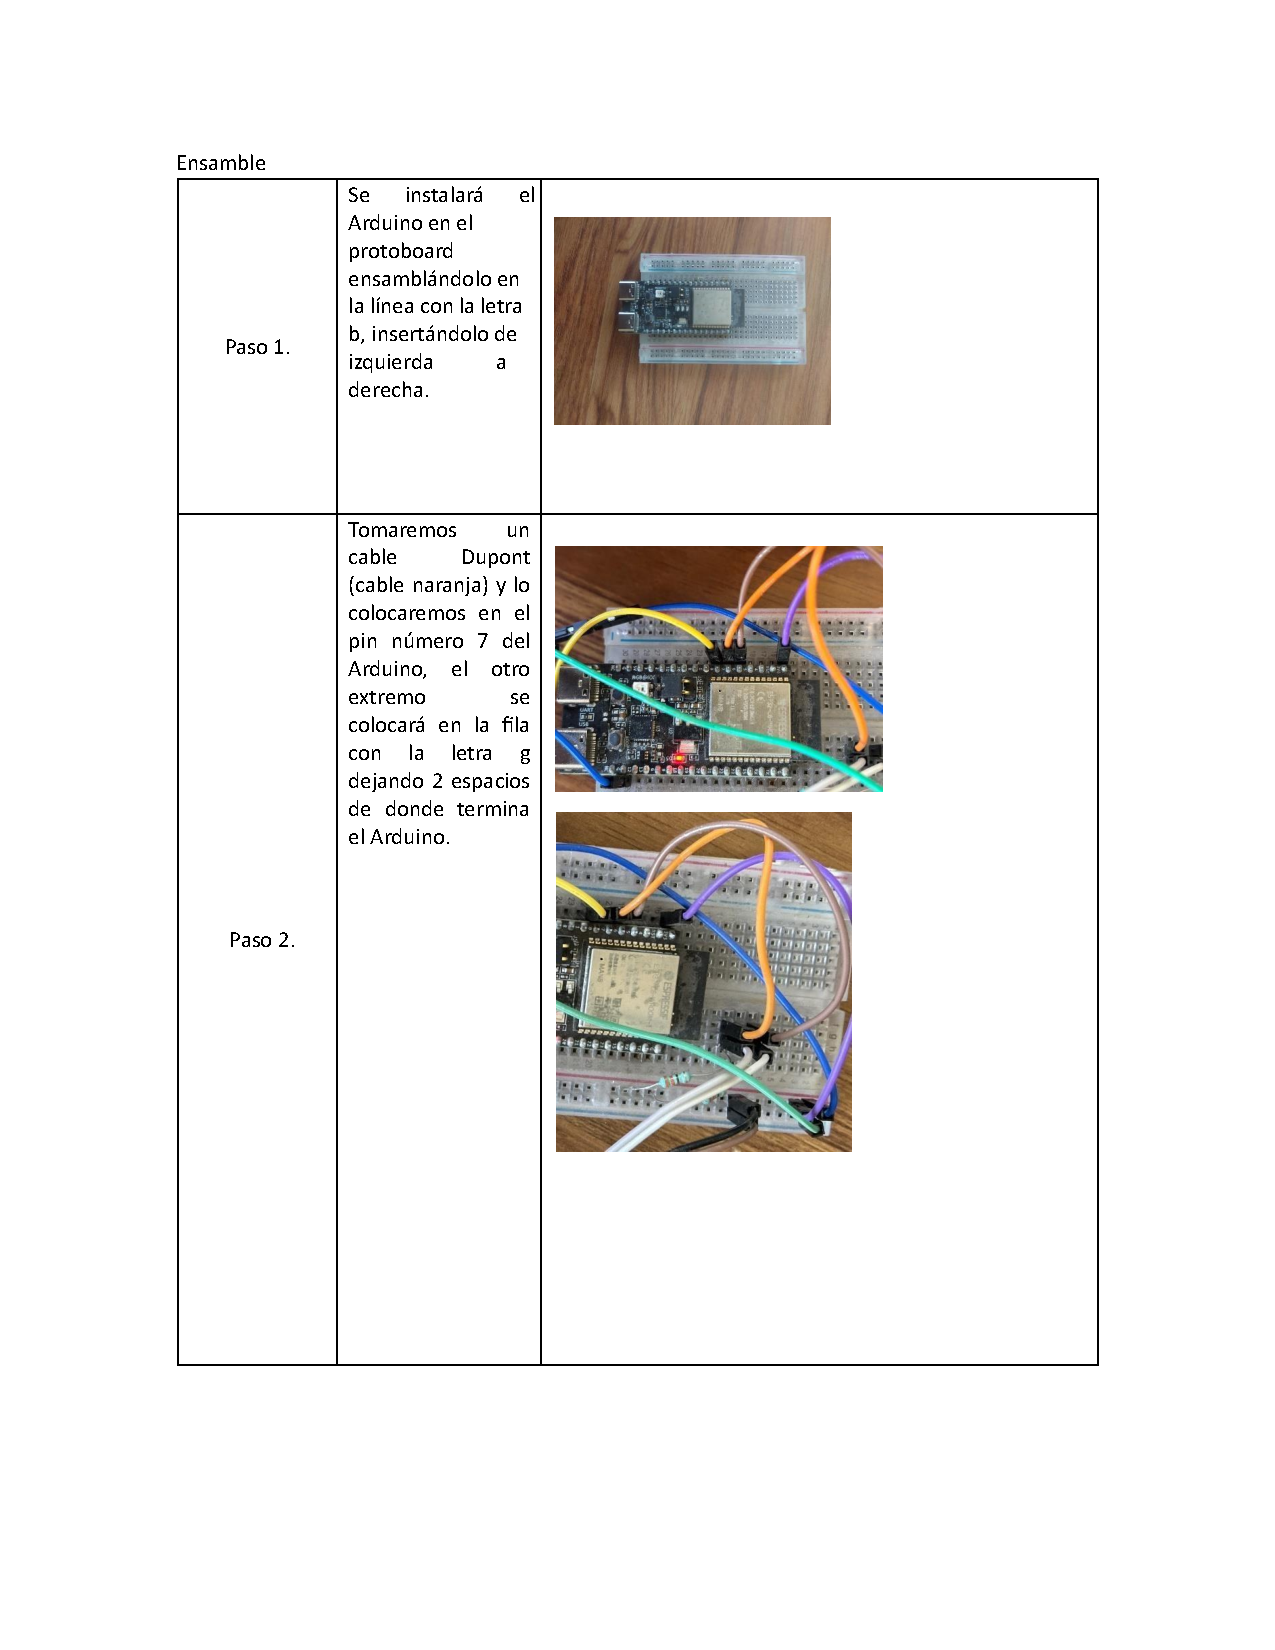
\includepdf[pages=-]{10/Img/ensamble.pdf}
    %%%%%%%%%%%%%%%%%%%%%%%%%%%%%%%%%%%%%%%%
    % \newpage
    % \bibliographystyle{ieeetr}
    % \bibliography{10/referencias}